\documentclass[dvipsnames, svgnames, x11names]{beamer}
\usepackage[T1]{fontenc}
\usepackage{bold-extra}
\usepackage{amsfonts, amsthm, amsmath, amssymb}
\usepackage{mathtools}
\usepackage{ulem}
\usepackage{bm}
\usepackage{minted}
\usemintedstyle{vs}
\usetheme{Madrid}
\usecolortheme{default}
\usepackage{multirow, multicol}
\usepackage{tikz, pgfplots}
\usetikzlibrary{arrows.meta, math, calc, quotes, intersections, angles, trees, shapes}
\pgfplotsset{compat=1.18}
\tikzstyle{block} = [rectangle, minimum width=4cm, minimum height=2cm, text centered, draw = black]
\tikzmath{\x1 = 2.5; \y1 = 3;}

\graphicspath{{../images}}

\title[HKUST Future-Ready Scholars]{HKUST Future-Ready Scholars}
\subtitle{Introduction to Game Programming using Python}
\author[Game Programming using Python]{Part 2}
\date[May 2024]{4 May 2024}
\titlegraphic{
\includegraphics[height=1cm]{ust.png}}

\begin{document}

\setbeamertemplate{page number in head/foot}{\insertframenumber /47}

\frame{\titlepage}

\begin{frame}[fragile]{Revision}
    \begin{center}
        Open a tab on your browser, then go to

        \href{https://www.kahoot.it/}{https://www.kahoot.it/}

        \

        \frame{
\includegraphics[width=0.75\textwidth]{Kahoot-Demo.png}}
    \end{center}
\end{frame}

\begin{frame}[fragile]{Files}
    \begin{center}
        All materials today are at:

        \href{https://bit.ly/ustidpo}{https://bit.ly/ustidpo}

        \

        \frame{
\includegraphics[width=0.75\textwidth]{Download.png}}

        %Download all files that belong to \textbf{Workshop 2} today.
    \end{center}
\end{frame}    

\begin{frame}[fragile]{Summary from Last Workshop}
    \begin{center}
        Let's look at what we learnt last time.
    \end{center}
\end{frame}

\begin{frame}[fragile]{Summary from Last Workshop}
    \begin{block}{Examples of valid integers}
        \begin{minted}[autogobble, tabsize=4, escapeinside=||]{python}
        a = 5  
        b = 1000000   
        c = -1984
        \end{minted}
    \end{block}
    \begin{block}{Examples of valid strings}
        \begin{minted}[autogobble, tabsize=4, escapeinside=||]{python}
        a = "5"
        b = "haha"   
        c = 'some words'
        \end{minted}
    \end{block}
    \begin{block}{Arithmetic Operators}
        Some basic and commonly-used operators:\\
        \centering
        \begin{tabular}{rlrl}
        \texttt{+}:& add & \texttt{-}:& minus,\\
        \texttt{*}:& multiply & \texttt{/}:& divide
        \end{tabular}
    \end{block}
\end{frame}

\begin{frame}[fragile]{Summary from Last Workshop}
\begin{block}{The \texttt{print()} statement}
\mint{py}{print(*objects)}

\fbox{\texttt{*objects}} - the things you want to print (put on the screen)
\end{block}

\begin{block}{The \texttt{input()} statement}
\mint{py}{input(prompt)}
where \fbox{\texttt{prompt}} is quite literally what it means. It prints the prompt, then returns the value inputted as a string.
\end{block}
\end{frame}

\begin{frame}[fragile]{Summary from Last Workshop}
\begin{block}{Comparison Operators}
There are 6 comparison operators:
\begin{center}
\begin{tabular}{|c|c|}\hline
Operator & Meaning\\\hline
\texttt{==} & equal to\\\hline
\texttt{>} & larger than\\\hline
\texttt{>=} & larger than or equal to\\\hline
\texttt{<} & smaller than\\\hline
\texttt{<=} & smaller than or equal to\\\hline
\texttt{!=} & not equal to\\\hline
\end{tabular}
\end{center}
\end{block}
\end{frame}

\begin{frame}[fragile]{Summary from Last Workshop}
\begin{block}{\texttt{if}, \texttt{elif} and \texttt{else}}
\texttt{if}, \texttt{elif} and \texttt{else} clauses are used to decide whether some code should be executed.
Whenever one is fulfilled, all others are ignored.
\begin{minted}[tabsize=4, escapeinside=||]{python}
if condition1: # if condition1 is true
    # Do something, ignore all elif and else below

elif condition2: # if condition2 is true
    # Do something, ignore all elif and else below

elif condition3: # if condition3 is true
    # Do something, ignore all elif and else below

else: # if all the conditions above are false
    # Do something
\end{minted}
\end{block}
\end{frame}

\begin{frame}[fragile]{Summary from Last Workshop}
\begin{block}{The \texttt{and} logic operator}
The \texttt{and} operator makes it so that both conditions have to be fulfilled in order for the code it is under to execute.
\end{block}
\begin{block}{The \texttt{or} logic operator}
The \texttt{or} operator makes it so that only 1 of the conditions have to be fulfilled in order for the code it is under to execute.
\end{block}
\begin{block}{The \texttt{not} logic operator}
The \texttt{not} operator reverses the condition is it attached to.
\end{block}
\begin{alertblock}{Multiple logic operators}
One can chain multiple logic operators together, but to be safe add brackets () to make sure the condition works as intended.
\end{alertblock}
\end{frame}

\begin{frame}[fragile]{Hangman}
    \begin{center}
        Let's start off with a simple game of Hangman.
    \end{center}
\end{frame}

\begin{frame}{World of Game Coding}
    \tikzstyle{block} = [rectangle, minimum width=4cm, minimum height=2cm, text centered, draw = black]
    \tikzmath{\x1 = 2.5; \y1 = 3;}
    
    \hspace{0.2\textwidth}\scalebox{0.5}{\begin{tikzpicture}
    \node (root) [block, fill = Cornsilk2] {Game (Software)};
    \node (program) [block, fill = LightSteelBlue] at ($(root) + (-\x1, -\y1)$) {Program (Code)};
    \node (mm) [block, fill = Cornsilk2] at ($(root) + (\x1, -\y1)$) {Multimedia};
    
    \node (func) [block, fill = LightSteelBlue] at ($(program) + (0, -\y1)$) {Functions};
    
    \node (if) [block, fill = LightSteelBlue] at ($(func) + (-\x1, -\y1)$) {Decision Making};
    \node (loop) [block, fill = LightSteelBlue] at ($(func) + (\x1, -\y1)$) {Loops};
    
    \node (io) [block, fill = LightSteelBlue] at ($(if) + (0, -\y1)$) {Input/Output};
    \node (var) [block, fill = LightSteelBlue] at ($(loop) + (0, -\y1)$) {Variables};
    
    \draw [->] (root.south) -- ++(0, -0.5) -- ++(-\x1, 0) -- (program.north);
    \draw [->] (root.south) -- ++(0, -0.5) -- ++(\x1, 0) -- (mm.north);
    
    \draw [->] (program.south) -- (func.north);
    
    \draw [->] (func.south) -- ++(0, -0.5) -- ++(-\x1, 0) -- (if.north);
    \draw [->] (func.south) -- ++(0, -0.5) -- ++(\x1, 0) -- (loop.north);
    
    \draw [->] (loop.south) -- ++(0, -0.5) -- ++(-2*\x1, 0) -- (io.north);
    \draw [->] (if.south) -- ++(0, -0.5) -- ++(2*\x1, 0) -- (var.north);
    \end{tikzpicture}}
\end{frame}
    
\begin{frame}{Contents} 
\begin{center}
    \scalebox{0.5}{\begin{tikzpicture}
    \node (program) [block, fill = LightSteelBlue] {Program (Code)};
    
    \node (func) [block, fill = LightSteelBlue] at ($(program) + (0, -\y1)$) {Functions};
    
    \node (if) [block, fill = LightSteelBlue] at ($(func) + (-\x1, -\y1)$) {Decision Making};
    \node (loop) [block, fill = LightSteelBlue] at ($(func) + (\x1, -\y1)$) {Loops};
    
    \node (io) [block, fill = LightSteelBlue] at ($(if) + (0, -\y1)$) {Input/Output};
    \node (var) [block, fill = DarkSeaGreen2] at ($(loop) + (0, -\y1)$) {Variables};
    
    \draw [->] (program.south) -- (func.north);
    
    \draw [->] (func.south) -- ++(0, -0.5) -- ++(-\x1, 0) -- (if.north);
    \draw [->] (func.south) -- ++(0, -0.5) -- ++(\x1, 0) -- (loop.north);
    
    \draw [->] (loop.south) -- ++(0, -0.5) -- ++(-2*\x1, 0) -- (io.north);
    \draw [->] (if.south) -- ++(0, -0.5) -- ++(2*\x1, 0) -- (var.north);
    \end{tikzpicture}}
\end{center}
\end{frame}

\begin{frame}[fragile]{More on Boolean values}
There are 2 Boolean values in existence: \texttt{True} and \texttt{False}.

The meaning of them are very similar to their English counterparts.

\begin{minted}[tabsize=4, escapeinside=||]{python}
status = True
if status:
    print("status is True")
else:
    print("status is False")
\end{minted}
\end{frame}

\begin{frame}[fragile]{More on Boolean values}
Another example:

\begin{minted}[tabsize=4, escapeinside=||]{python}
game_over = False
if not game_over:
    print("Continue your game!")
else:
    print("Game Over!")
\end{minted}
\end{frame}

\begin{frame}[fragile]{Lists}
Imagine you have a bunch of variables you want to store.
For example, if you have a bunch of people's names.
\begin{minted}[tabsize=4, escapeinside=||]{python}
name0 = "Chris Wong"
name1 = "Desmond Tsoi"
name2 = "Phoebe Mok"
name3 = "Nancy Ip"
\end{minted}
That is annoying to store and access.

\pause What if instead, we store it in the same thing, as a... \pause list?
\end{frame}

\begin{frame}[fragile]{Lists}
\begin{minted}[tabsize=4, escapeinside=||]{python}
names = ["Chris Wong", "Desmond Tsoi",
         "Phoebe Mok", "Nancy Ip"]
\end{minted}

\

Lists are declared by surrounding the items with [ ], and separating each item with a comma.

\end{frame}

\begin{frame}[fragile]{Lists}
What we are going to learn with lists:

\begin{itemize}
    \item Getting elements
    \item Editing elements
    \item List with \texttt{print()}
    \item Length of a list
    \item Appending an element
    \item \texttt{in} operator
\end{itemize}
\end{frame}

\begin{frame}[fragile]{Lists}

We can get the name from a list by getting the corresponding item.

How? With list[index].

The first item in the list is the 0$^{\text{th}}$ item, second is 1$^{\text{st}}$ item, etc... 

We call this zero-indexing.\\

{\tiny Note: Some programming languages use one-indexing instead.\\[-1em]

\hspace{2.5em} If you approach another programming language, be careful.}
\end{frame}

\begin{frame}[fragile]{Lists}
\begin{minted}[tabsize=4, escapeinside=||]{python}
names = ["Chris Wong", "Desmond Tsoi",
         "Phoebe Mok", "Nancy Ip"]
print(names[0], names[1], names[2], names[3]) 
# Output:|\pause| Chris Wong Desmond Tsoi Phoebe Mok Nancy Ip
\end{minted}
\end{frame}

\begin{frame}[fragile]{Lists}
Another example:
\begin{minted}[tabsize=4, escapeinside=||]{python}
# Indices: 0  1  2  3  4  5
numbers = [0, 1, 1, 2, 3, 5]
print(numbers[0], numbers[1], numbers[2],
      numbers[3], numbers[4], numbers[5]) 
# Output: 0 1 1 2 3 5

print(numbers)
# Output: [0, 1, 1, 2, 3, 5]
\end{minted}
\end{frame}

\begin{frame}[fragile]{Lists}
One more example in the context of Hangman:
\begin{minted}[tabsize=4, escapeinside=||]{python}
# Indices:    0    1    2    3    4    5
word_list = ["p", "y", "t", "h", "o", "n"]
print(word_list[0], word_list[1], word_list[2],
      word_list[3], word_list[4], word_list[5]) 
# Output: p y t h o n

print(word_list)
# Output: ['p', 'y', 't', 'h', 'o', 'n']
\end{minted}
\end{frame}

\begin{frame}[fragile]{Lists}
To edit an element of a list, assign the new value to the correct index. \pause
\begin{minted}[tabsize=4, escapeinside=||]{python}
numbers = [0, 1, 1, 2, 3, 5]
print(numbers) # [0, 1, 1, 2, 3, 5]
numbers[1] = 100 # Edit the second element (index 1)
print(numbers)  
# Output: |\pause| [0, 100, 1, 2, 3, 5]
\end{minted}
\end{frame}

\begin{frame}[fragile]{Lists}
Another example in the context of Hangman:
\begin{minted}[tabsize=4, escapeinside=||]{python}
word_list = ["p", "y", "t", "h", "o", "n"]
print(word_list) # ['p', 'y', 't', 'h', 'o', 'n']
word_list[3] = "a" # Edit the fourth element (index 3)
print(word_list)  
# Output: |\pause| ['p', 'y', 't', 'a', 'o', 'n']
\end{minted}
\end{frame}

\begin{frame}[fragile]{Lists}
To get the length of a list, we can use the \texttt{len()} function. \pause
\begin{minted}[tabsize=4, escapeinside=||]{python}
numbers = [0, 1, 1, 2, 3, 5] |\pause|
print(len(numbers)) # 6 
word_list = ["p", "y", "t", "h", "o", "n"] |\pause|
print(len(word_list)) # 6
\end{minted}
\end{frame}

\begin{frame}[fragile]{Lists}
To add an element to the end to a list, we use the \texttt{append(value)} list function. \pause
\begin{minted}[tabsize=4, escapeinside=||]{python}
numbers = [0, 1, 1, 2, 3, 5]
print(numbers, "length:", len(numbers)) 
# Output: [0, 1, 1, 2, 3, 5] length: 6
numbers.append(100) # Add 100 to the end of the list
print(numbers, "length:", len(numbers))
# Output:|\pause| [0, 1, 1, 2, 3, 5, 100] length: 7
\end{minted}
\end{frame}

\begin{frame}[fragile]{Lists}
Another example in the context of Hangman:
\begin{minted}[tabsize=4, escapeinside=||]{python}
word_list = ["p", "y", "t", "h", "o", "n"]
print(word_list, "length:", len(word_list)) 
# Output: ['p', 'y', 't', 'h', 'o', 'n'] length: 6
word_list.append("a") # Add "a" to the end of the list
print(word_list, "length:", len(word_list))  
# Output: |\pause| ['p', 'y', 't', 'h', 'o', 'n', 'a'] length: 7
\end{minted}
\end{frame}

\begin{frame}[fragile]{Lists}
We can check if an element is in a list with the \texttt{in} operator.\pause

\begin{minted}[tabsize=4, escapeinside=||]{python}
numbers = [0, 1, 1, 2, 3, 5]
if 0 in numbers:
    print("0 is in numbers.") # This line is run
else:
    print("0 is not in numbers.")
if 8 in numbers:
    print("8 is in numbers.")
else:
    print("8 is not in numbers.") # This line is run
\end{minted}
\end{frame}

\begin{frame}[fragile]{Lists}
Another example in the context of Hangman:

\begin{minted}[tabsize=4, escapeinside=||]{python}
word_list = ["p", "y", "t", "h", "o", "n"]
if "y" in word_list:
    print("y is in the word list.")
else:
    print("y is not in the word list.")
if "a" in word_list:
    print("a is in the word list.")
else:
    print("a is not in the word list.")
\end{minted}
\end{frame}

\addtocounter{framenumber}{-1}

\begin{frame}[fragile]{Lists}
Another example in the context of Hangman:
    
\begin{minted}[tabsize=4, escapeinside=||]{python}
word_list = ["p", "y", "t", "h", "o", "n"]
if "y" in word_list:
    print("y is in the word list.") # This line is run
else:
    print("y is not in the word list.")
if "a" in word_list:
    print("a is in the word list.")
else:
    print("a is not in the word list.")
\end{minted}
\end{frame}

\addtocounter{framenumber}{-1}

\begin{frame}[fragile]{Lists}
Another example in the context of Hangman:
    
\begin{minted}[tabsize=4, escapeinside=||]{python}
word_list = ["p", "y", "t", "h", "o", "n"]
if "y" in word_list:
    print("y is in the word list.") # This line is run
else:
    print("y is not in the word list.")
if "a" in word_list:
    print("a is in the word list.")
else:
    print("a is not in the word list.") # This line is run
\end{minted}
\end{frame}

\begin{frame}[fragile]{More about the \texttt{in} operator}
The \texttt{in} operator works very similarly when applied to strings.
\begin{minted}[tabsize=4, escapeinside=||]{python}
word = "python"
if "y" in word:
    print("y is in the word.") # This line is run
else:
    print("y is not in the word.")
if "a" in word:
    print("a is in the word.")
else:
    print("a is not in the word.") # This line is run
\end{minted}
\end{frame}

\begin{frame}[fragile]{More about the \texttt{in} operator}
You can combine the \texttt{not} and \texttt{in} operators.
\begin{minted}[tabsize=4, escapeinside=||]{python}
word = "python"
if "a" not in word:
    print("a is not in the word.")
else:
    print("a is in the word.")
word_list = ["U", "S", "T"]
if "u" not in word_list:
    print("u is not in the list.")
else:
    print("u is in the list.")
\end{minted}
\end{frame}

\addtocounter{framenumber}{-1}

\begin{frame}[fragile]{More about the \texttt{in} operator}
You can combine the \texttt{not} and \texttt{in} operators.
\begin{minted}[tabsize=4, escapeinside=||]{python}
word = "python"
if "a" not in word:
    print("a is not in the word.") # This line is run
else:
    print("a is in the word.")
word_list = ["U", "S", "T"]
if "u" not in word_list:
    print("u is not in the list.")
else:
    print("u is in the list.")
\end{minted}
\end{frame}

\addtocounter{framenumber}{-1}

\begin{frame}[fragile]{More about the \texttt{in} operator}
You can combine the \texttt{not} and \texttt{in} operators.
\begin{minted}[tabsize=4, escapeinside=||]{python}
word = "python"
if "a" not in word:
    print("a is not in the word.") # This line is run
else:
    print("a is in the word.")
word_list = ["U", "S", "T"]
if "u" not in word_list:
    print("u is not in the list.") # This line is run
else:
    print("u is in the list.")
\end{minted}
\end{frame}

\begin{frame}{Contents}
    \begin{center}\scalebox{0.5}{
        \begin{tikzpicture}
        \node (program) [block, fill = LightSteelBlue] {Program (Code)};
        
        \node (func) [block, fill = LightSteelBlue] at ($(program) + (0, -\y1)$) {Functions};
        
        \node (if) [block, fill = LightSteelBlue] at ($(func) + (-\x1, -\y1)$) {Decision Making};
        \node (loop) [block, fill = DarkSeaGreen2] at ($(func) + (\x1, -\y1)$) {Loops};
        
        \node (io) [block, fill = LightSteelBlue] at ($(if) + (0, -\y1)$) {Input/Output};
        \node (var) [block, fill = LightSteelBlue] at ($(loop) + (0, -\y1)$) {Variables};
        
        \draw [->] (program.south) -- (func.north);
        
        \draw [->] (func.south) -- ++(0, -0.5) -- ++(-\x1, 0) -- (if.north);
        \draw [->] (func.south) -- ++(0, -0.5) -- ++(\x1, 0) -- (loop.north);
        
        \draw [->] (loop.south) -- ++(0, -0.5) -- ++(-2*\x1, 0) -- (io.north);
        \draw [->] (if.south) -- ++(0, -0.5) -- ++(2*\x1, 0) -- (var.north);
        \end{tikzpicture}}
    \end{center}
\end{frame}

\begin{frame}[fragile]{Loops}
What do you do if you want to do something repeatedly in code? \pause 
\begin{minted}[tabsize=4, escapeinside=||]{python}
print("Count:", 0)
print("Count:", 1)
print("Count:", 2)
print("Count:", 3)
print("Count:", 4)
print("Count:", 5)
print("Count:", 6)
print("Count:", 7)
print("Count:", 8)
print("Count:", 9)
print("Done.")
\end{minted} 
\pause 
Let's turn this into a loop.
\end{frame}

\begin{frame}[fragile]{Loops - \texttt{while}}
Example:
\begin{minted}[tabsize=4, escapeinside=||]{python}
i = 0 # Initialising i as 0
while i < 10:
    print("Count:", i)
    i = i + 1
print("Done.")
\end{minted}
Let's run through it together.
\end{frame}

\addtocounter{framenumber}{-1}

\begin{frame}[fragile]{Loops - \texttt{while}}
Example:
\begin{minted}[tabsize=4, escapeinside=||]{python}
i = 0
while i < 10: # i is 0, which is smaller than 10
    print("Count:", i)
    i = i + 1
print("Done.")
\end{minted}
\end{frame}

\addtocounter{framenumber}{-1}

\begin{frame}[fragile]{Loops - \texttt{while}}
Example:
\begin{minted}[tabsize=4, escapeinside=||]{python}
i = 0
while i < 10: 
    print("Count:", i) # Count: 0
    i = i + 1
print("Done.")
\end{minted}
\end{frame}

\addtocounter{framenumber}{-1}

\begin{frame}[fragile]{Loops - \texttt{while}}
Example:
\begin{minted}[tabsize=4, escapeinside=||]{python}
i = 0
while i < 10: 
    print("Count:", i)
    i = i + 1 # i goes from 0 to 1, then we go back up
print("Done.")
\end{minted}
\end{frame}

\addtocounter{framenumber}{-1}

\begin{frame}[fragile]{Loops - \texttt{while}}
Example:
\begin{minted}[tabsize=4, escapeinside=||]{python}
i = 0
while i < 10: # i is 1, which is smaller than 10
    print("Count:", i)
    i = i + 1
print("Done.")
\end{minted}
\end{frame}

\addtocounter{framenumber}{-1}

\begin{frame}[fragile]{Loops - \texttt{while}}
Example:
\begin{minted}[tabsize=4, escapeinside=||]{python}
i = 0
while i < 10: 
    print("Count:", i) # Count: 1
    i = i + 1
print("Done.")
\end{minted}
\end{frame}

\addtocounter{framenumber}{-1}

\begin{frame}[fragile]{Loops - \texttt{while}}
Example:
\begin{minted}[tabsize=4, escapeinside=||]{python}
i = 0
while i < 10: 
    print("Count:", i)
    i = i + 1 # i goes from 1 to 2, then we go back up
print("Done.")
\end{minted}
\end{frame}

\addtocounter{framenumber}{-1}

\begin{frame}[fragile]{Loops - \texttt{while}}
Example:
\begin{minted}[tabsize=4, escapeinside=||]{python}
i = 0
while i < 10: # i is 2, which is smaller than 10
    print("Count:", i)
    i = i + 1
print("Done.")
\end{minted}
\end{frame}

\addtocounter{framenumber}{-1}

\begin{frame}[fragile]{Loops - \texttt{while}}
Example:
\begin{minted}[tabsize=4, escapeinside=||]{python}
i = 0
while i < 10: 
    print("Count:", i) # Count: 2
    i = i + 1
print("Done.")
\end{minted}
\end{frame}

\addtocounter{framenumber}{-1}

\begin{frame}[fragile]{Loops - \texttt{while}}
Example:
\begin{minted}[tabsize=4, escapeinside=||]{python}
i = 0
while i < 10: 
    print("Count:", i)
    i = i + 1 # i goes from 2 to 3, then we go back up
print("Done.")
\end{minted}
\end{frame}

\addtocounter{framenumber}{-1}

\begin{frame}[fragile]{Loops - \texttt{while}}
Example:
\begin{minted}[tabsize=4, escapeinside=||]{python}
i = 0
while i < 10: # i is 3, which is smaller than 10
    print("Count:", i)
    i = i + 1
print("Done.")
\end{minted}

This goes on and on\dots
\end{frame}

\addtocounter{framenumber}{-1}

\begin{frame}[fragile]{Loops - \texttt{while}}
Example:
\begin{minted}[tabsize=4, escapeinside=||]{python}
i = 0
while i < 10: # i is 9, which is smaller than 10
    print("Count:", i)
    i = i + 1
print("Done.")
\end{minted}
\end{frame}

\addtocounter{framenumber}{-1}

\begin{frame}[fragile]{Loops - \texttt{while}}
Example:
\begin{minted}[tabsize=4, escapeinside=||]{python}
i = 0
while i < 10: 
    print("Count:", i) # Count: 9
    i = i + 1
print("Done.")
\end{minted}
\end{frame}

\addtocounter{framenumber}{-1}

\begin{frame}[fragile]{Loops - \texttt{while}}
Example:
\begin{minted}[tabsize=4, escapeinside=||]{python}
i = 0
while i < 10: 
    print("Count:", i)
    i = i + 1 # i goes from 9 to 10, then we go back up
print("Done.")
\end{minted}
\end{frame}

\addtocounter{framenumber}{-1}

\begin{frame}[fragile]{Loops - \texttt{while}}
Example:
\begin{minted}[tabsize=4, escapeinside=||]{python}
i = 0
while i < 10: # i is 10, which is NOT smaller than 10
    print("Count:", i)
    i = i + 1
print("Done.")
\end{minted}
\end{frame}

\addtocounter{framenumber}{-1}

\begin{frame}[fragile]{Loops - \texttt{while}}
Example:
\begin{minted}[tabsize=4, escapeinside=||]{python}
i = 0
while i < 10:
    print("Count:", i)
    i = i + 1
print("Done.") # "Done." is printed
\end{minted}
\end{frame}

\begin{frame}[fragile]{Loops - \texttt{while}}
Example:
\begin{minted}[tabsize=4, escapeinside=||]{python}
i = 0
while i < 10:
|\textvisiblespace\textvisiblespace\textvisiblespace\textvisiblespace|print("Count:", i)
|\textvisiblespace\textvisiblespace\textvisiblespace\textvisiblespace|i = i + 1
print("Done.")
\end{minted}
\begin{block}{Indentation}
Just like \texttt{if}-clauses, the indentation must be consistent for statements in the loop.
This also applies to \texttt{for} loops, which we will get into very soon.
\end{block}
\end{frame}

\begin{frame}[fragile]{Loops - \texttt{while}}
Example in the context of Hangman:
\begin{minted}[tabsize=4, escapeinside=||]{python}
max = 6
wrong_guess = 0
while wrong_guess < max:
    print("You have", max - wrong_guess, "guesses left.")
    # Some more code to decide if the guess is wrong
\end{minted}
\end{frame}

\begin{frame}[fragile]{Loops - \texttt{for}}
Example:
\begin{minted}[tabsize=4, escapeinside=||]{python}
for i in range(10):
    print("Count:", i)
print("Done.")
\end{minted}
\begin{block}{Python \texttt{range}}
Python \texttt{range} is a thing of mystery. When you do \texttt{range(n)}, where \texttt{n} is an integer, Python generates a \textit{range} of integers from 0 to \texttt{n} - 1.
\end{block}
\end{frame}

\begin{frame}[fragile]{Loops - \texttt{for}}
Example:
\begin{minted}[tabsize=4, escapeinside=||]{python}
for i in range(10):
    print("Count:", i)
print("Done.")
\end{minted}

\ 

\tikzstyle{forArrow} = [single arrow, draw=none, fill=green!50, anchor=base, align=center,text width=1cm]
\begin{tikzpicture}
    \node (A) [forArrow] {\texttt{i=0}};
    \node (B) [forArrow, right of=A, xshift=0.75cm] {\texttt{i=1}};
    \node (C) [forArrow, right of=B, xshift=0.75cm] {\texttt{i=2}};
    \node (D) [draw=none, right of=C, xshift=0.25cm] {$\cdots$};
    \node (E) [forArrow, right of=D, xshift=0.05cm] {\texttt{i=8}};
    \node (F) [forArrow, right of=E, xshift=0.75cm] {\texttt{i=9}};
\end{tikzpicture}
\end{frame}

\begin{frame}[fragile]{Loops - \texttt{for}}
\begin{minted}[tabsize=4, escapeinside=||]{python}
for i in range(10):
    print("Count:", i)
print("Done.")
\end{minted}

\

is equivalent to

\

\begin{minted}[tabsize=4, escapeinside=||]{python}
i = 0
while i < 10:
    print("Count:", i)
    i = i + 1
print("Done.")
\end{minted}

Both loops go from 0 to 9, and give identical output.
\end{frame}

\begin{frame}[fragile]{Loops - \texttt{for}}
Another example:
\begin{minted}[tabsize=4, escapeinside=||]{python}
for i in range(3):
    print(i * i) # Print the square
# Output:|\pause| 0 |\pause|
#         1 |\pause|
#         4
\end{minted}
\end{frame}

\begin{frame}[fragile]{Loops - \texttt{for}}
Let's combine lists with a for loop.
\begin{minted}[tabsize=4, escapeinside=||]{python}
word = ["p", "y", "t", "h", "o", "n"]
for i in range(len(words)):
    print(word[i]) # Print word[i]
# Output:|\pause| p |\pause|
#         y |\pause|
#         t |\pause|
#         h |\pause|
#         o |\pause|
#         n
\end{minted}
\pause This is one way we go through a list.
\end{frame}

\begin{frame}[fragile]{Loops - \texttt{for}}
Instead of using the index, there is another way to go through a list:
\begin{minted}[tabsize=4, escapeinside=||]{python}
word = ["p", "y", "t", "h", "o", "n"]
for i in word:
    print(i) # Print the element
# Output:|\pause| p |\pause|
#         y |\pause|
#         t |\pause|
#         h |\pause|
#         o |\pause|
#         n
\end{minted}
\pause The output is identical to the previous example.
\end{frame}

\begin{frame}[fragile]{Summary}
\begin{block}{Boolean values}
There are only 2 Boolean values: \texttt{True} and \texttt{False}.

They are very similar to their English counterpart and \texttt{True}/\texttt{False} are opposites.
\end{block}
\begin{block}{Lists}
Lists are represented with [ ] to hold multiple variables, where the $i^{\text{th}}$ item is at index $i - 1$.\\
\end{block}
\begin{block}{Lists with functions}
If a list is called \texttt{l}, one can:
\begin{itemize}
    \item print the list with \texttt{print(l)}.
    \item get the length of \texttt{l} with \texttt{len(l)}.
    \item get/edit the element at index \texttt{i} with \texttt{l[i]}.
\end{itemize}
\end{block}
\end{frame}

\begin{frame}[fragile]{Summary}
\begin{block}{List functions}
If a list is called \texttt{l}, one can:
\begin{itemize}
    \item append a value \texttt{v} to \texttt{l} with \texttt{l.append(v)}.
    \item use the \texttt{in} operator to check if a value \texttt{v} is in a list.
    \item[] e.g.: \texttt{if v in l:}
\end{itemize}
\end{block}

\begin{block}{\texttt{in} operator}
You can use \texttt{in} operator for strings too, and even combine it with the \texttt{not} operator.
\begin{minted}[tabsize=4]{python}
w = "HKUST"
if "H" not in w:
    print("No H.")
else:
    print("Yes H.") # This line is run.
\end{minted}
\end{block}
\end{frame}

\begin{frame}[fragile]{Summary}
\begin{block}{\texttt{while} loops}
\begin{minted}[tabsize=4, escapeinside=||]{python}
while condition:
    # Do code
\end{minted}
Code in the \texttt{while} block are run while the condition is fulfilled.\\
Do make sure that the \texttt{while} loop can be exited.
\end{block}
\end{frame}

\begin{frame}[fragile]{Summary}
\begin{block}{\texttt{for} loops and \texttt{range}}
\begin{minted}[tabsize=4, escapeinside=||]{python}
n = 5 # Example
for i in range(n):
    # Do code with each number from 0 to n - 1
\end{minted}
\texttt{range(n)} returns a range of integers that starts from 0 and ends at \texttt{n} - 1.
\end{block}

\begin{block}{\texttt{for} loops and lists}
\begin{minted}[tabsize=4, escapeinside=||]{python}
l = [...] # A list with items
for i in l:
    # Do code with each item in the list
\end{minted}
\texttt{for} loops can be directly applied onto lists.
\end{block}
\end{frame}

\begin{frame}[fragile]{Google Colab}
    \begin{center}
        Login to your Gmail account.

        \

        Then head to

        \href{https://colab.research.google.com/}{https://colab.research.google.com/}
    \end{center}
\end{frame}

\begin{frame}[fragile]{Jupyter Notebook}
    \begin{center}
        Now upload your Jupyter Notebook file with \textbf{Files $\rightarrow$ Open Notebook}.
    
        \

        \frame{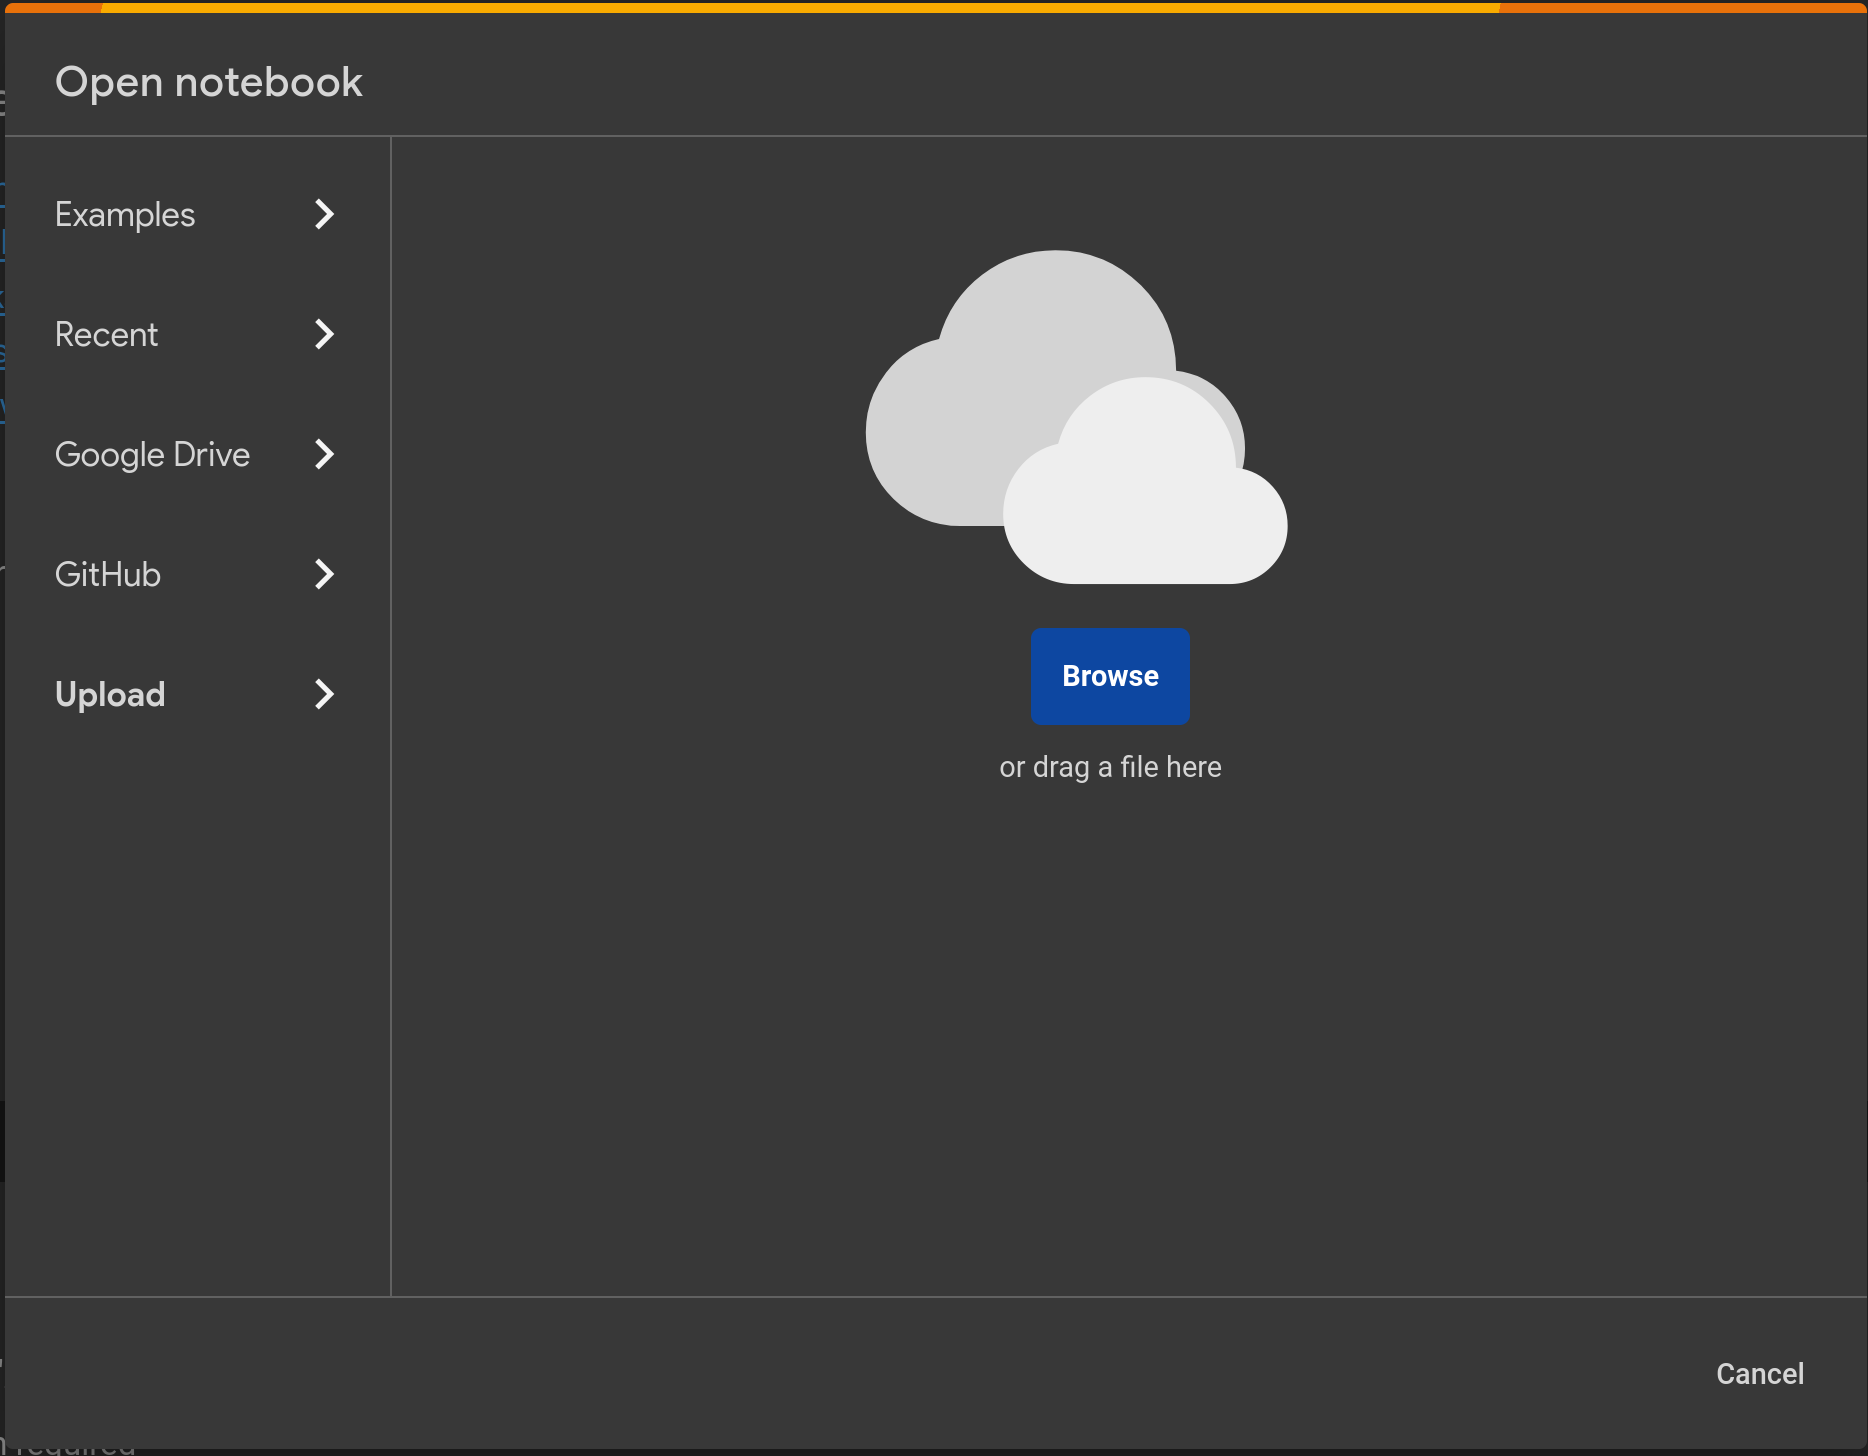
\includegraphics[width=0.5\textwidth]{Upload.png}}

        Upload the file \textbf{Hangman.ipynb}.
    
    \end{center}
\end{frame}

\begin{frame}[fragile]{Using Jupyter Notebook}
    You can type your code in these blocks. We call these blocks code cells.

    \begin{center}
        \frame{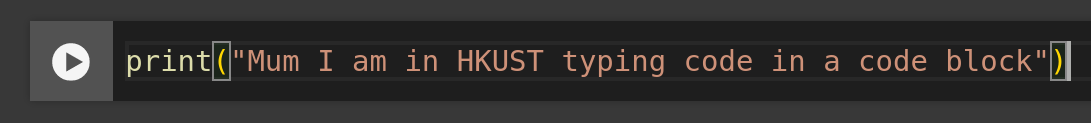
\includegraphics[width=0.5\textwidth]{Use1.png}}
    \end{center}

    \

    You can run a code cell with the button on the left.

    \begin{center}
        \frame{
\includegraphics[width=0.5\textwidth]{Use2.png}}
    \end{center}
\end{frame}

\begin{frame}{ \ }
	\begin{center}
		The End\\
		Thank you!
	\end{center}
\end{frame}






%%%-------------------------ADDITIONAL CONTENT-------------------------%%%
\setcounter{framenumber}{0}
\setbeamertemplate{page number in head/foot}{S-\insertframenumber /S-15}











\begin{frame}{Additional content}
	\begin{center}
		Here are some additional content that we didn't think we would have time to mention in the workshop.
	\end{center}
\end{frame}

\begin{frame}{Contents} 
\begin{center}
    \scalebox{0.5}{\begin{tikzpicture}
    \node (program) [block, fill = LightSteelBlue] {Program (Code)};
    
    \node (func) [block, fill = LightSteelBlue] at ($(program) + (0, -\y1)$) {Functions};
    
    \node (if) [block, fill = LightSteelBlue] at ($(func) + (-\x1, -\y1)$) {Decision Making};
    \node (loop) [block, fill = LightSteelBlue] at ($(func) + (\x1, -\y1)$) {Loops};
    
    \node (io) [block, fill = LightSteelBlue] at ($(if) + (0, -\y1)$) {Input/Output};
    \node (var) [block, fill = DarkSeaGreen2] at ($(loop) + (0, -\y1)$) {Variables};
    
    \draw [->] (program.south) -- (func.north);
    
    \draw [->] (func.south) -- ++(0, -0.5) -- ++(-\x1, 0) -- (if.north);
    \draw [->] (func.south) -- ++(0, -0.5) -- ++(\x1, 0) -- (loop.north);
    
    \draw [->] (loop.south) -- ++(0, -0.5) -- ++(-2*\x1, 0) -- (io.north);
    \draw [->] (if.south) -- ++(0, -0.5) -- ++(2*\x1, 0) -- (var.north);
    \end{tikzpicture}}
\end{center}
\end{frame}

\begin{frame}[fragile]{Lists}
To insert an element to a particular position in a list, we use the \texttt{insert()} list function.

The \texttt{insert(i, value)} inserts the \texttt{value} at index \texttt{i}, and push everything after to the right. \pause
\begin{minted}[tabsize=4, escapeinside=||]{python}
numbers = [0, 1, 1, 2, 3, 5]
print(numbers, "length:", len(numbers)) 
# Output: [0, 1, 1, 2, 3, 5] length: 6
numbers.insert(2, 100) # Add 100 to index 2 of the list
print(numbers, "length:", len(numbers))  
# Output:|\pause| [0, 1, 100, 1, 2, 3, 5] length: 7
numbers.insert(7, 200)|\pause| # Same as numbers.append(200)
print(numbers, "length:", len(numbers))  
# Output:|\pause| [0, 1, 100, 1, 2, 3, 5, 200] length: 8
\end{minted}
\end{frame}

\begin{frame}[fragile]{Lists}
To remove an element from a list, we use the \texttt{remove()} list function.

The \texttt{remove(value)} function removes the \textbf{first} occurence of \texttt{value}. \pause
\begin{minted}[tabsize=4, escapeinside=||]{python}
numbers = [0, 1, 1, 2, 3, 5]
print(numbers, "length:", len(numbers)) 
# Output: [0, 1, 1, 2, 3, 5] length: 6
numbers.remove(1) # Remove the first occurence of number 1
print(numbers, "length:", len(numbers))
# Output:|\pause| [0, 1, 2, 3, 5] length: 5
\end{minted}
\end{frame}

\begin{frame}[fragile]{Lists}
The \texttt{reverse()} list function reverses a list's contents. \pause

\begin{minted}[tabsize=4, escapeinside=||]{python}
numbers = [0, 1, 1, 2, 3, 5]
print(numbers, "length:", len(numbers)) 
# Output: [0, 1, 1, 2, 3, 5] length: 6
numbers.reverse() # Reverse the list
print(numbers, "length:", len(numbers)) 
# Output:|\pause| [5, 3, 2, 1, 1, 0] length: 6
print(numbers[0])
# Output:|\pause| 5
\end{minted}
\end{frame}

\begin{frame}[fragile]{Lists}
The \texttt{count(item)} list function counts the number of occurence of \texttt{item} in a list. \pause

\begin{minted}[tabsize=4, escapeinside=||]{python}
numbers = [0, 1, 1, 2, 3, 5]
print(numbers.count(1)) 
# Output:|\pause| 2
print(numbers.count(100)) 
# Output:|\pause| 0
\end{minted}
\end{frame}

\begin{frame}[fragile]{Lists}
The \texttt{index(item)} list function finds the index of the first occurence of \texttt{item} in a list. \pause

\begin{minted}[tabsize=4, escapeinside=||]{python}
numbers = [0, 1, 1, 2, 3, 5]
print(numbers.index(1)) 
# Output:|\pause| 1
print(numbers.index(5)) 
# Output:|\pause| 5
print(numbers.index(100))
# Output:|\pause| No output, error, 100 is not in the list
\end{minted}
\end{frame}

\begin{frame}[fragile]{Lists}
Combining \texttt{in} and \texttt{list.index()}: \pause

\begin{minted}[tabsize=4, escapeinside=||]{python}
numbers = [0, 1, 1, 2, 3, 5]
if 5 in numbers:
    print("The index of 5 in the list is", numbers.index(5))
# Output:|\pause| The index of 5 in the list is 5
\end{minted}
\end{frame}

\begin{frame}[fragile]{Lists}
The \texttt{sort()} list function sorts a list's contents. \pause

\begin{minted}[tabsize=4, escapeinside=||]{python}
numbers = [6, 5, 1, 2, 3]
print(numbers, "length:", len(numbers)) 
# Output: [6, 5, 1, 2, 3] length: 5
print(numbers[0])
# Output: 6
numbers.sort() # Sort the list
print(numbers, "length:", len(numbers)) 
# Output:|\pause| [1, 2, 3, 5, 6] length: 5
print(numbers[0])
# Output:|\pause| 1
\end{minted}
\end{frame}

\begin{frame}{Contents} 
\begin{center}
    \scalebox{0.5}{\begin{tikzpicture}
    \node (program) [block, fill = LightSteelBlue] {Program (Code)};
    
    \node (func) [block, fill = LightSteelBlue] at ($(program) + (0, -\y1)$) {Functions};
    
    \node (if) [block, fill = LightSteelBlue] at ($(func) + (-\x1, -\y1)$) {Decision Making};
    \node (loop) [block, fill = DarkSeaGreen2] at ($(func) + (\x1, -\y1)$) {Loops};
    
    \node (io) [block, fill = LightSteelBlue] at ($(if) + (0, -\y1)$) {Input/Output};
    \node (var) [block, fill = LightSteelBlue] at ($(loop) + (0, -\y1)$) {Variables};
    
    \draw [->] (program.south) -- (func.north);
    
    \draw [->] (func.south) -- ++(0, -0.5) -- ++(-\x1, 0) -- (if.north);
    \draw [->] (func.south) -- ++(0, -0.5) -- ++(\x1, 0) -- (loop.north);
    
    \draw [->] (loop.south) -- ++(0, -0.5) -- ++(-2*\x1, 0) -- (io.north);
    \draw [->] (if.south) -- ++(0, -0.5) -- ++(2*\x1, 0) -- (var.north);
    \end{tikzpicture}}
\end{center}
\end{frame}

\begin{frame}[fragile]{Loops - \texttt{while}}
We can also apply boolean values to \texttt{while} loops.
\begin{minted}[tabsize=4, escapeinside=||]{python}
equal_to_5 = False
count = 0
while not equal_to_5:
    if count == 5:
        equal_to_5 = True
    count = count + 1
print("Done.") # "Done." is printed
\end{minted}
\end{frame}

\begin{frame}[fragile]{Summary}
The \texttt{range} in Python does not always have to start at 0.
\begin{minted}[tabsize=4, escapeinside=||]{python}
for i in range(2, 5):
    print(i)
# Output:|\pause| 2
#         3
#         4
\end{minted}
\begin{block}{Custom \texttt{range}}
Given \texttt{range(a, b)}, a \texttt{for} loop will iterate from \texttt{a} to \texttt{b - 1}.
\end{block}
\end{frame}

\begin{frame}[fragile]{Summary}
\begin{block}{List functions}
If a list is called \texttt{l}, one can:
\begin{itemize}
    \item insert a value \texttt{v} to \texttt{l} at index \texttt{i} with \texttt{l.insert(i, v)}.
    \item remove the first occurence of a value \texttt{v} with \texttt{l.remove(v)}.
    \item reverse the list with \texttt{l.reverse()}.
    \item count the occurence of value \texttt{v} with \texttt{l.count(v)}.
    \item get the index of the first occurence of a value \texttt{v} with \texttt{l.index(v)}.
    \item sort the list with \texttt{l.sort()}.
\end{itemize}
\end{block}

\end{frame}

\begin{frame}[fragile]{Summary}
\begin{block}{Boolean conditions of \texttt{while}}
You can apply boolean conditions to \texttt{while} loops.
\begin{minted}[tabsize=4, escapeinside=||]{python}
status = True # Or False, or a condition with variables
while status: # Can also add "not"
    # Do something
\end{minted}
\end{block}

\begin{block}{Custom \texttt{range}}
Given \texttt{range(a, b)}, a \texttt{for} loop will iterate from \texttt{a} to \texttt{b - 1}.
\begin{minted}[tabsize=4, escapeinside=||]{python}
sum = 0
for i in range(100, 102):
    sum = sum + i
print(sum) # Output: 201
\end{minted}
\end{block}
    
\end{frame}

\begin{frame}{ \ }
	\begin{center}
		End of Additional Contents\\
		Made in \LaTeX\\
		Last updated: 29 Apr 2024
	\end{center}
\end{frame}

\end{document}
